\documentclass[tikz,border=3.14pt]{standalone}
\usepackage{amsmath}
%\usetikzlibrary{3d,decorations.text,shapes.arrows,positioning,fit,backgrounds,arrows}

\begin{document}

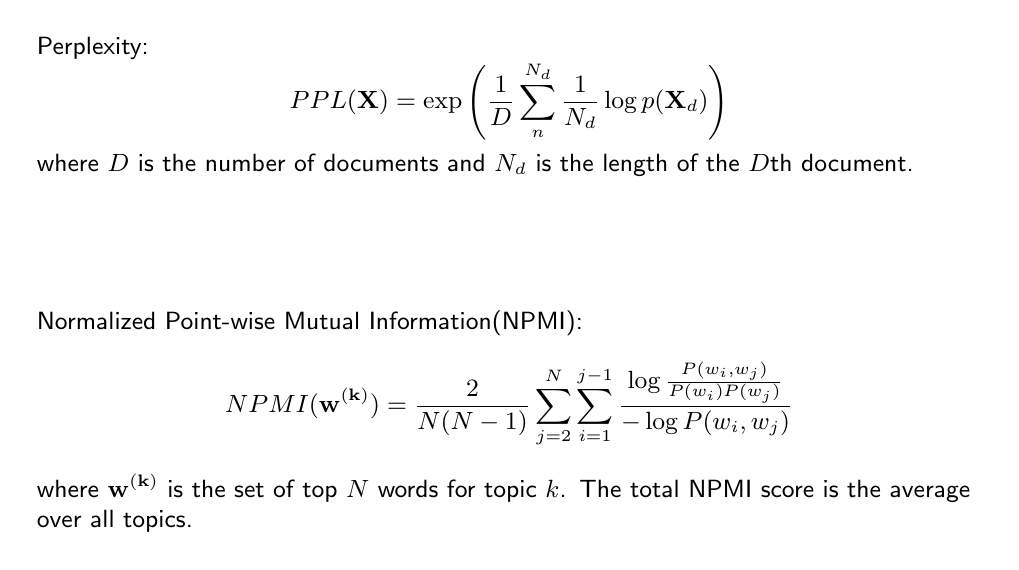
\begin{tikzpicture}[font=\sffamily\small,scale=2]

\node[text width=12cm] at (0,1) {
Perplexity:
\[ PPL({\bf X}) = \exp\left(\frac{1}{D}\sum_n^{N_d}\frac{1}{N_d}\log p({\bf X}_d)\right) \]
where $D$ is the number of documents and $N_d$ is the length of the $D$th document.};

\node[text width=12cm] at (0,-1) {
Normalized Point-wise Mutual Information(NPMI):
\[ NPMI({\bf w^{(k)}}) = \frac{2}{N(N-1)}\sum_{j=2}^N\sum_{i=1}^{j-1}\frac{\log\frac{P(w_i,w_j)}{P(w_i)P(w_j)}}{-\log P(w_i,w_j)} \]
where ${\bf w^{(k)}}$ is the set of top $N$ words for topic $k$. The total NPMI score is the average over all topics.};

\end{tikzpicture}

\end{document}
